
% Infrastruktur
% Implementierung
	% Ordnerstruktur
	% Patterns
		% PageObject
		% PageFactory
	% Architektur
		% TestRunners
	% Testbeschreibung

\chapter{Umsetzung}
\label{sec:umsetzung}

\section{Prozess}
Der Prozess wurde equivalent aufgesetzt, wie es im \cref{sec:konzept:prozess} \nameref{sec:konzept:prozess} beschrieben wurde.

\begin{figure}[H]
	\centering
	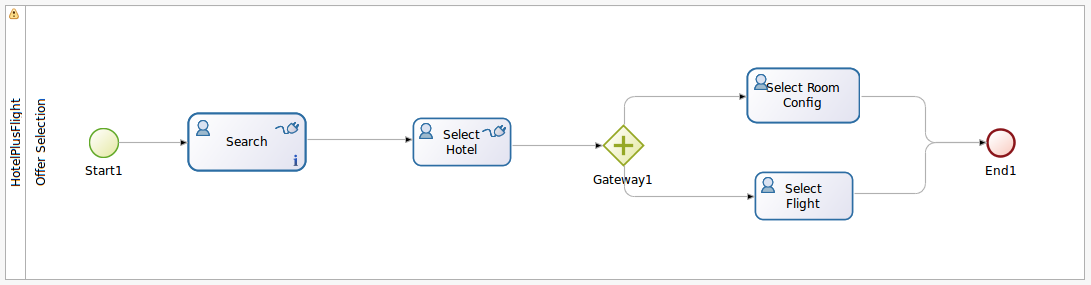
\includegraphics[width=1\textwidth]{images/umsetzung-prozess.png}
	\caption{Prozess im Bonita}
	\label{fig:umsetzung:prozess}
\end{figure}
Das Icon oben Links in den Task signalisiert, dass es sich dabei um einen Human Task handelt und eine Benutzerinteraktion erforderlich ist. Das Bild oben rechts in den Task zeigt an, dass es einen Connector auf dem Task gibt.

\section{Business Data Models und Pool Variables}
Als \glspl{bdm} wurden folgende Modelle definiert:
\begin{table}[H] 
	\caption{Business Data Models}
	\centering
	\label{sec:umsetzung:bdm:bdm}
	
	\begin{tabular}{ | l | l | c | } 
		\hline
		\textbf{Name} & \textbf{Type} & \textbf{Multiple} \\ \hline 
		\multicolumn{3}{|c|}{\textbf{HotelPlusFlightSearch}} \\ \hline 
		destination & string & \\ \hline
		departure & string & \\ \hline
		adults & integer & \\ \hline
		fromDate & date & \\ \hline
		toDate & date & \\ \hline
		id & string & \\ \hline
		\multicolumn{3}{|c|}{\textbf{HotelPlusFlightResults}} \\ \hline 
		hotels & HotelPlusFlightResultHotel & x \\ \hline
		\multicolumn{3}{|c|}{\textbf{HotelPlusFlightResultHotel}} \\ \hline 
		name & string & \\ \hline
		price & string & \\ \hline
		image & string & \\ \hline
		roomConfigs & HotelPlusFlightRoomConfig & x \\ \hline
		flights & HotelPlusFlightFlightResult & x \\ \hline
		id & string & \\ \hline
		\multicolumn{3}{|c|}{\textbf{HotelPlusFlightRoomConfig}} \\ \hline 
		roomType & string & \\ \hline
		mealType & string & \\ \hline
		id & string & \\ \hline
		\multicolumn{3}{|c|}{\textbf{HotelPlusFlightFlightResult}} \\ \hline 
		airline & string & \\ \hline
		fromAirport & string & \\ \hline
		toAirport & string & \\ \hline
		flight1FromTime & string & \\ \hline
		flight1ToTime & string & \\ \hline
		flight2FromTime & string & \\ \hline
		flight2ToTime & string & \\ \hline
		id & string & \\ \hline
	\end{tabular} 
\end{table}

Auf der Poolebene wurde für jedes \gls{bdm} eine Pool Variable erstellt. Der Name der Variable entspricht dem \gls{bdm}, beginnt jedoch mit einem kleinen Buchstaben.
\begin{table}[H] 
	\caption{Pool Variables}
	\centering
	\label{sec:umsetzung:bdm:poolvariable}
	
	\begin{tabular}{ | l | l | c | } 
		\hline
		\textbf{Name} & \textbf{BDM} \\ \hline 
		hotelPlusFlightSearch & HotelPlusFlightSearch \\ \hline
		hotelPlusFlightResults & HotelPlusFlightResults \\ \hline
		hotelPlusFlightResultHotel & HotelPlusFlightResultHotel \\ \hline
		hotelPlusFlightRoomConfig & HotelPlusFlightRoomConfig \\ \hline
	 	hotelPlusFlightFlightResult & HotelPlusFlightFlightResult \\ \hline
	\end{tabular} 
\end{table}
\section{Forms}
Die Formulare wurden bereits für die Mockups im \cref{sec:konzept:mockups} \nameref{sec:konzept:mockups} erstellt und konnten wiederverwendet werden.

\section{Connectors}
